\documentclass[11pt]{scrartcl}
\usepackage{graphicx}
\graphicspath{{./}}
\usepackage[sexy]{evan}
\usepackage[normalem]{ulem}
\usepackage{hyperref}
\usepackage{mathtools}
\hypersetup{
    colorlinks=true,
    linkcolor=blue,
    filecolor=magenta,      
    urlcolor=cyan,
    pdftitle={Overleaf Example},
    pdfpagemode=FullScreen,
    }

\renewcommand{\baselinestretch}{1.5}

\addtolength{\oddsidemargin}{-0.4in}
\addtolength{\evensidemargin}{-0.4in}
\addtolength{\textwidth}{0.8in}
% \addtolength{\topmargin}{-0.2in}
% \addtolength{\textheight}{1in} 

\usepackage{pgfplots}
\pgfplotsset{compat=1.15}
\usepackage{mathrsfs}
\usetikzlibrary{arrows}
\setlength\parindent{0pt}

\begin{document}
	\title{Handout Basic Math for Computer Science} % Beginner
	\date{\today}
	\author{Azzam L. H. (Math IG: Azzam L. H.)}
	\maketitle
	Handout ini hanya bersifat rangkuman :) jadi belajar dari tempat lain juga ya :)
    \section{Logika Dasar}
    	\begin{enumerate}
    	    \item $A \land B$ dibaca $A$ dan $B$.
    	    \item $A \lor B$ dibaca $A$ atau $B$.
    	    \item $A \equiv B$ dibaca $A$ ekuivalen $B$ (untuk logika).
    	    \item $\exists x$ dibaca ada $x$ atau terdapat $x$.
    	    \item $\forall x$ dibaca untuk semua $x$.
    	    \item $A \implies B$ dibaca
    	    \begin{enumerate}
    	        \item $A$ hanya jika $B$,
    	        \item $B$ jika $A$,
    	        \item $A$ mengimplikasikan $B$,
    	        \item $A$ menyebabkan $B$,
    	        \item jika $A$ maka $B$.
    	    \end{enumerate}
    	    \item $A \Longleftarrow B$ dibaca $A$ jika $B$ (kebalikannya $\implies$).
    	    \item $A \iff B$ dibaca $A$ jika dan hanya jika $B$. Definisinya adalah $A \iff B \equiv (A \implies B) \land (A \Longleftarrow B)$.
    	\end{enumerate}
    	Apa bedanya $A \implies B$ dan $A \iff B$? Kalau $A \implies B$ berarti agar pernyataan benar haruslah $B$ benar, $A$ bisa salah atau benar. Kalau $A \iff B$, agar pernyataan benar, haruslah $A$ dan $B$ sama-sama benar atau sama-sama salah. Contohnya:
    	\begin{itemize}
    	    \item Jika sekarang hujan, maka saya tidak pergi. (Baik sekarang hujan ataupun tidak hujan, bisa saja saya tidak pergi, jadi tidak pengaruh).
    	    \item Klise tapi ya.... : Saya bergerak jika dan hanya jika saya tidak diam :).
    	\end{itemize}
    	\section{Himpunan}    	
    	Misalkan $A$ dan $B$ adalah dua himpunan.
    	\begin{enumerate}
    	    \item $\phi$ atau $\{\}$ adalah himpunan kosong atau himpunan yang tidak mempunyai elemen.
    	    \item Banyak elemen dari $A$ dinotasikan dengan $|A|$ (dibaca "kardinalitas dari $A$") atau $n(A)$ .
    	    \item $x \in A$ dibaca $x$ elemen dari $A$.
    	    \item $A \subseteq B$ dibaca $A$ subset dari $B$ atau $A$ himpunan bagian dari $B$.
    	    \item $A \subset B$ dibaca $A$ adalah proper subset dari $B$. Bedanya dengan $\subseteq$?\\
    	    $\subset$ itu mirip $<$ dimana tidak mungkin $A \subset A$, tetapi $\subseteq$ itu mirip $\le$ karena mungkin $A \subseteq A$.
    	    \item $A \cup B$ dibaca $A$ union $B$ atau $A$ gabung $B$.
    	    \item $A \cap B$ dibaca $A$ intersection $B$ atau $A$ irisan $B$.
    	    \item $A^c$ atau $A'$ dibaca $A$ komplemen.
    	    \item $|A \cup B| = |A|+|B|-|A \cap B|$.
    	\end{enumerate}
    \section{Aljabar}
     \subsection{Floor and Ceiling}
    Definisikan $\floor{x}$ (floor x) sebagai bilangan bulat terbesar yang kurang dari sama dengan $x$. Simpelnya, $\floor{x}$ dapat dikatakan sebagai "pembulatan ke bawah". Contoh: $\floor{\pi}=3$, $\floor{2}=2$, $\floor{10,51}=10$, $\floor{-1,5}=-2$.
    
    Definisikan $\ceiling{x}$ (ceiling x) sebagai bilangan bulat terkecil yang lebih dari sama dengan $x$. Simpelnya, $\ceiling{x}$ dapat dikatakan sebagai "pembulatan ke atas". Contoh: $\ceiling{\pi}=4$, $\ceiling{2}=2$, $\ceiling{10,51}=11$, $\ceiling{-1,5}=-1$.
    
    Beberapa properti:
    \begin{enumerate}
        \item $\floor{x}=\ceiling{x}$ untuk $x \in \ZZ$.
        \item $\floor{x}=\ceiling{x}-1$ untuk $x \not \in \ZZ$.
        \item $\floor{x} \le  x < \floor{x}+1$ untuk $x \in \RR$.
        \item $\ceiling{x}-1 < x \le \ceiling{x}$ untuk $x \in \RR$.
        \item $\floor{a+x}=a+\floor{x}$ dan $\ceiling{a+x}=a+\ceiling{x}$ untuk $a\in \ZZ$ dan $x \in \RR$.
    \end{enumerate}
    
    \section{Teori Bilangan}
    \subsection{Sifat-sifat Penjumlahan dan Perkalian Dua Bilangan Bulat}
        \begin{enumerate}
            \item Bilangan Ganjil ± Bilangan Ganjil = Bilangan Genap 
            \item Bilangan Ganjil ± Bilangan Genap = Bilangan Ganjil 
            \item Bilangan Genap ± Bilangan Ganjil = Bilangan Ganjil 
            \item Bilangan Genap ± Bilangan Genap = Bilangan Genap 
            \item Bilangan Ganjil $\times$ Bilangan Ganjil = Bilangan Ganjil 
            \item Bilangan Ganjil $\times$ Bilangan Genap = Bilangan Genap 
            \item Bilangan Genap $\times$ Bilangan Ganjil = Bilangan Genap 
            \item Bilangan Genap $\times$ Bilangan Genap = Bilangan Genap
        \end{enumerate}
        Dari sifat-sifat perkalian dua bilangan akan didapat bahwa bilangan genap tidak mungkin membagi 
        bilangan ganjil sedangkan bilangan ganjil mungkin membagi bilangan genap. 
        \subsection{Keterbagian}
        Untuk bilangan bulat $a \neq 0$ serta bilangan bulat $b,c,x$ dan $y$, notasikan $a \mid b$ sebagai $a$ membagi $b$. Lalu, $a$ dan $b$ relatif prima atau $a$ dan $b$ koprima (coprime) jika dan hanya jika $FPB(a,b)=1$.
        \begin{enumerate}
            \item Kita dapat menyatakan semua bilangan bulat $c = pq+r$ untuk suatu bilangan bulat $q$ dimana $0 \le r < q$. Jadi, saat $c$ dibagi $p$, maka hasil baginya adalah $q$ dan sisa baginya adalah $r$.
            \item Terdapat suatu bilangan bulat $x$ dimana $a \mid b \iff b=ax$.
            \item $a \mid a$.
            \item $a \mid 0$.
            \item $1 \mid a$.
            \item $a \mid b \implies a \mid bc$.
            \item Untuk $a,b \neq 0$ maka $ab \mid c \implies a \mid c \text{ dan } b \mid c$.
            \item $a \mid b \text{ dan } b \mid c \implies a \mid c$.
            \item $a \mid b \text{ dan } a \mid c \implies a \mid bx + cy$.
            \item Untuk $x \neq 0$ maka $a \mid b \iff xa \mid xb$.
            \item $a \mid b$ dan $b \neq 0$ maka $|a| \le |b|$.
            \item $a \mid bc$ dan $FPB(a,b)=1$ maka $a\mid c$.
        \end{enumerate}
        \subsection{Uji habis dibagi}
        Trik yang suatu saat dapat membuat hidup anda bahagia wkwkwk. Semua rumus ini dapat dibuktikan dengan aritmatika modular.
        \begin{enumerate}
            \item Bilangan $x$ genap jika dan hanya jika digit terakhir $x$ genap.
            \item $3 \mid x$ jika dan hanya jika jumlah digit-digitnya habis dibagi $3$. Contohnya 2931 habis dibagi 3 karena $2+9+3+1=15$ habis dibagi 3.
            \item $9 \mid x$ jika dan hanya jika jumlah digit-digitnya habis dibagi $9$.
            \item $x$ habis dibagi 5 jika dan hanya jika digit terakhir $x$ adalah $0$ atau $5$.
            \item $x$ habis dibagi 11 jika dan hanya jika jumlah selang-seling (alternate sums) dari digit-digitnya habis dibagi 11. Contoh: 945351 habis dibagi 11 karena $9-4+5-3+5-1=11$ habis dibagi 11. 121 habis dibagi 11 karena $1-2+1=0$ habis dibagi 11.
        \end{enumerate}
        
        \subsection{Aritmatika Modular}
        Untuk suatu bilangan asli $m$ dan bilangan bulat $a,b,c$ dan $d$, notasikan $m\mid a-b \iff a \equiv b \mod m$ (dibaca $a$ kongruen $b$ modulo $m$). Simpelnya $a \equiv b \mod m$ adalah $a$ dibagi $m$ bersisa $b$. Contohnya $5 \equiv 2 \mod 3$. $13 \equiv 3 \mod 5$. $10 \equiv -2 \mod 12$.
        \begin{enumerate}
            \item $a \equiv a \mod m$.
            \item $a \equiv 0 \mod m \iff m\mid a$.
            \item $a \equiv b \mod m \iff b \equiv a \mod m$.
            \item $a \equiv b \mod m \text{ dan } b \equiv c \mod m \implies a \equiv c \mod m$.
            \item Jika $a \equiv b \mod m$ dan $d\mid m$ maka $a \equiv b \mod d$.
            \item Untuk semua bilangan asli $k$, $a \equiv b \mod m \iff a^k \equiv b^k \mod m$.
            \item $a \equiv b \mod m \text{ dan } c \equiv d \mod m \implies a+c \equiv b+d \mod m$.
            \item $a \equiv b \mod m \text{ dan } c \equiv d \mod m \implies ac \equiv bd \mod m$.
            \item $\forall k\in \ZZ^+, (am+b)^k \equiv b^k \mod m$.
            \item Jika $ca \equiv cb \mod m$ dengan $FPB(c,m)=1$, maka $a \equiv b \mod m$.
        \end{enumerate}
        
        Penggunaan sifat nomor 8 dapat dimodifikasi sehingga menjadi konsep \textbf{Chinese Remainder Theorem}.
        
    \subsection{Inverse Modulo}
    Misalkan bilangan bulat $a$, $x$ dan bilangan bulat positif $m$. Kita sebut $x$ adalah inverse dari $a \mod m$ jika dan hanya jika $gcd(a,m)=1$ dan $ax \equiv 1 \mod m$.
    
    \subsection{Bilangan Prima Serta Trik-trik Modulo Umum}
    Bilangan prima adalah bilangan asli yang hanya dapat dibagi dirinya sendiri dan angka 1. 
    
    Bilangan bukan prima dan bukan 1 disebut bilangan komposit.
    
    1 bukan bilangan prima dan bukan pula bilangan komposit. 
    
    Untuk bilangan prima $p$ dan bilangan bulat $n$.
    \begin{enumerate}
        \item Bilangan prima genap hanya ada satu buah, yaitu 2.
        \item Dari definisi bilangan prima $p$, karena $p$ tak terbagi oleh $2$ dan $5$, maka tak ada bilangan prima yang berakhiran $0$.
        \item Untuk sembarang bilangan prima $p$ berlaku $p \mid n$ atau $gcd(p,n)=1$.
        \item $p \mid n^2$ jika dan hanya jika $p \mid n$.
        \item $p \mid ab \iff p \mid a \text{ atau } p \mid b$.
        \item Untuk $p > 3$, kita punya bentuk $p = 6k \pm 1$ untuk suatu bilangan asli $k$.
        \item (Sieve of Erastosthenes) 
        Faktor prima terkecil $t$ dari bilangan komposit $n$ selalu $t \le \sqrt{n}$.
        \end{enumerate}
        
    Lalu, beberapa trik-trik modulo umum:
    \begin{enumerate}
        \item Pada sistem persamaan bulat, tinjau modulo 3, 4, 5, 7, atau modulo 11 nya.
        \item Untuk bilangan bulat $n$ selalu terjadi $n^2 \equiv 1 \mod 4$, $n^2 \equiv 1 \mod 3$. Peninjauan terhadap modulo lain juga bisa, namun tidak terlalu umum.
    \end{enumerate}
    
    \subsection{Basis Bilangan}
    Basis bilangan adalah sistem bilangan yang menyatakan banyaknya digit atau kombinasi dari digit-digit yang menyatakan sebuah bilangan.
    
    Secara umum, bilangan $a$ dalam basis $n > 0$ yaitu $(a)_n$ mempunyai bentuk (yang setara dengan nilai basis 10):
    $$(c_kc_{k-1}\dotsc_1c_0)_n = c_{k}n^k + c_{k-1}n^{k-1}+\dots+c_1n^{1}+c_0n^{0}$$
    
    Secara umum bahkan kita telah memakai sistem basis tersebut untuk basis 10. Misalkan 123 dapat dinyatakan sebagai $123 = 1\cdot 10^2 + 2\cdot 10^1 + 1\cdot 10^0$
    
    Lalu, berikut merupakan contoh untuk bilangan basis selain 10 misalnya: 
    \begin{itemize}
        \item Bilangan basis 2 atau bilangan biner yang digit-digitnya terdiri dari $\{0,1\}$. Misalkan $1001_2$ dalam biner yang setara dengan $9$ atau $1001_2 = 9$ karena $1001_2 = 1\cdot 2^3+0\cdot 2^2+0\cdot 2^1+1\cdot 2^0 = 9$. 
        \item Bilangan basis 3 yang digit-digitnya terdiri dari $\{0,1,2\}$. Misalkan $211_3 = 22$ karena $211_3 = 2\cdot 3^2+ 1\cdot 3^1+ 1\cdot 3^0 = 22$.
        \item Bilangan basis 16 atau heksadesimal yang digit-digitnya terdiri dari $\{0,1,2,\dots,9,A,B,\dots,F\}$. Misalkan $5F_{16} = 95$ karena $5F_{16} = 5 \cdot 16^1 + (15)\cdot 16^0 = 95$.
    \end{itemize}
    
    \subsection{FPB dan KPK dua bilangan}
        Secara matematis FPB (atau gcd - greatest common divisors) dan KPK (atau lcm - least common multiples) dari dua bilangan bulat positif $a$ dan $b$ 
        didefinisikan sebagai:
        $$FPB(a,b) = gcd(a,b) = p_1^{\min\{a_1,b_1\}}\cdot p_2^{\min\{a_2,b_2\}} \cdot \ldots \cdot p_n^{\min\{a_n,b_n\}}$$
        $$KPK(a,b) = lcm(a,b) =p_1^{\max\{a_1,b_1\}}\cdot p_2^{\max\{a_2,b_2\}} \cdot \ldots \cdot p_n^{\max\{a_n,b_n\}}$$
        dimana kedua bilangan tersebut dapat difaktorisasi prima menjadi
        $a=p_1^{a_1}\cdot p_2^{a_2}\cdot \ldots \cdot p_n^{a_n}$ dan $b=p_1^{b_1}\cdot p_2^{b_2} \cdot \ldots \cdot p_n^{b_n}$, dengan $p_1,p_2,\dots,p_n$ adalah bilangan prima berbeda, serta $a_1,a_2,\dots,a_n,b_1,b_2,\dots,b_n$ adalah bilangan bulat non-negatif.
        
        Dari definisi tersebut mudah dibuktikan bahwa
        $$FPB(a,b) \cdot KPK(a,b) = ab.$$
        
        Perlu dicatat, bahwa $a$ dan $b$ tidak boleh bernilai nol. Untuk $a,b$ yang bernilai negatif, didefinisikan $FPB(a,b) = FPB(|a|,|b|)$.
        \subsubsection{Algoritma Euclid}
        Pada dasarnya algoritma ini bertumpu pada sebuah teorema:
        $$FPB(a,b) = FPB(a,b-a)$$
        
        \subsection{Fungsi yang Melibatkan Faktor Bilangan}
        Misalkan $a$ dapat difaktorisasi prima seperti sebelumnya yaitu $a=p_1^{a_1}\cdot p_2^{a_2}\cdot \ldots \cdot p_n^{a_n}$.
        \subsubsection{Banyaknya Faktor Positif}
        Fungsi $d(a)$ didefinisikan sebagai banyaknya faktor atau pembagi positif dari $a$ dengan
        $$d(a) = (a_1+1)(a_2+1)\cdot \ldots \cdot (a_n+1).$$
        
        Contoh: Banyaknya faktor positif dari $12= 2^2 \cdot 3^1$ adalah $d(12)=(2+1)(1+1)=6$ dengan pembagi positifnya adalah $1,2,3,4,6,12$ (ada 6 faktor positif.)
        
        \subsubsection{Jumlah Faktor Positif}
        Fungsi $\sigma (a)$ didefinisikan sebagai banyaknya faktor atau pembagi positif dari $a$ dengan
        $$\sigma (a) = (p_1^0+p_1^1+p_1^2+\dots+p_1^{a_1})(p_2^0+p_2^1+p_2^2+\dots+p_2^{a_2})\cdot \ldots \cdot (p_n^0+p_n^1+p_n^2+\dots+p_n^{a_n}).$$
        
        Contoh: Jumlah faktor atau pembagi positif dari $12= 2^2 \cdot 3^1$ adalah $d(12)=(2^0+2^1+2^2)(3^0+3^1)=28$ yang setara dengan penjumlahan secara manualnya, yaitu $2^03^0+2^03^1+2^13^0+2^13^1+2^23^0+2^23^1=28.$
        
        \subsubsection{Banyaknya Bilangan Relatif Prima}
        \begin{remark*}
        	     Bilangan $b$ dikatakan relatif prima dengan $a$ jika dan hanya jika $FPB(a,b)=1$.
        	\end{remark*}
         Definisikan fungsi Euler Totient Phi $\phi(b)$ sebagai banyaknya bilangan bulat positif $n$ yang kurang dari sama dengan $b$ dimana $n$ relatif prima dengan $b$. Rumus eksplisit untuk menghitung fungsi ini adalah
        $$\phi(n) = a\left(1-\dfrac{1}{p_1}\right)\left(1-\dfrac{1}{p_2}\right)\dots\left(1-\dfrac{1}{p_n}\right).$$
        
        Contoh: $\phi(4)=4(1-\frac{1}{2})=2$ karena ada 2 bilangan yang realtif prima dengan 4, yaitu 1 dan 3.
        
        Catatan: Untuk semua bilangan prima $p$, nilai $\phi(p) = p-1$. (Silakan dibuktikan sendiri :D)
        
        \subsection{Euler's Theorem on Modulo}
        Untuk bilangan asli $a$ dan $n$ yang saling relatif prima kita punya
        $$a^{\phi(n)} \equiv 1 \mod n.$$
        
        \subsection{Fermat's Little Theorem}
        Teorema ini merupakan kasus khusus dari Euler's Theorem saat $n$ prima sehingga $\phi(n)=n-1$. Untuk bilangan prima $p$, kita punya
        $$a^{p-1} \equiv 1 \mod p.$$
        
        \subsection{Wilson's theorem}
        Untuk suatu bilangan asli $p$, kita punya $p$ adalah bilangan prima jika dan hanya jika
        $$(p-1)! \equiv -1 \mod p.$$
   
    \section{Kombinatorika}
    Seluruh bagian kombinatorika ini disadur dari buku Diktat Pembinaan Olimpiade Matematika Dasar versi 5.2 karya Pak Eddy Hermanto.
    
     Notasikan $n!=n \times (n-1) \times (n-2) \times \dots \times 3 \times 2 \times 1$ (dibaca $n$ faktorial) dengan $1!=0!=1$.
        
        \subsection{Kombinasi dan Permutasi}
        Permutasi $k$ unsur dari $n$ unsur adalah (urutan diperhatikan)
        $$_nP_K = P_k^n = \dfrac{n!}{(n-k)!}.$$
        Kombinasi $k$ unsur dari $n$ unsur adalah (urutan tak diperhatikan)
        $${n \choose k}=_nC_K = C_k^n = \dfrac{n!}{k!(n-k)!}.$$
        
        \subsection{Permutasi Siklis}
        $n$ objek ditaruh mengelilingi lingkaran maka banyak cara menyusunnya adalah
        $$P_{siklis} =\dfrac{n!}{n} = (n-1)!$$
        
        \subsection{Stars and Bars}
        Banyaknya solusi bulat non-negatif $(x_1,x_2,\dots,x_k)$ dari sistem persamaan $x_1+x_2+\dots+x_k=n$ adalah
        $${n+k-1 \choose k-1}.$$
        Banyaknya solusi bulat positif $(x_1,x_2,\dots,x_k)$ dari sistem persamaan $x_1+x_2+\dots+x_k=n$ adalah
        $${n-1 \choose k-1}.$$
    
    \subsection{Percobaan}
Misalkan kita melempar sekeping uang logam, maka kegiatan ini disebut dengan percobaan. Hasil 
percobaan yang didapat biasanya adalah munculnya sisi gambar, $G$, atau munculnya sisi tulisan, $T$. 
Sedangkan jika kita melempar sebuah dadu, maka hasil percobaan yang didapat adalah mata dadu 1, 
2, 3, 4, 5 atau 6. 

\subsection{Ruang Contoh atau Ruang Sampel} 
Ruang contoh atau ruang sampel adalah himpunan dari semua hasil percobaan yang mungkin. Ruang 
contoh atau ruang sampel biasanya dilambangkan dengan $S$ yang dalam teori himpunan disebut 
dengan himpunan semesta. 
Pada percobaan melempar uang logam, ruang sampelnya adalah $\{G, T\}$ sedangkan pada percobaan
melempar satu buah dadu, ruang sampelnya adalah $\{1, 2, 3, 4, 5, 6\}$. 
Jika $\{G, T\}$ adalah ruang sampel, maka anggota-anggota dari ruang sampel tersebut disebut titik
contoh. Titik contoh dari $\{G, T\}$ adalah $G$ dan $T$. Pada percobaan melempar satu buah dadu, titik 
sampel yang didapat ada 6 yaitu 1, 2, 3, 4, 5, 6 sedangkan jika melempar dua buah dadu akan didapat
36 buah titik contoh, yaitu $(1, 1), (1, 2), (1, 3), \dots , (6, 6)$. 

\subsection{Kejadian}
Kejadian atau peristiwa (event) adalah himpunan bagian dari ruang contoh yang dapat berupa
kejadian sederhana maupun kejadian majemuk. Kejadian sederhana adalah suatu kejadian yang
hanya mempunyai sebuah titik contoh. Jika suatu kejadian memiliki lebih dari satu titik contoh 
disebut dengan kejadian majemuk. 
Kejadian munculnya mata dadu satu $\{1\}$ pada percobaan melempar sebuah dadu adalah contoh 
kejadian sederhana. Contoh dari kejadian majemuk adalah munculnya mata dadu genap pada 
percobaan melempar sebuah dadu. 
    
\subsection{Peluang Suatu Kejadian}
Menghitung peluang dengan pendekatan frekuensi 
Dari suatu percobaan yang dilakukan sebanyak $n$ kali, ternyata kejadian $A$ munculnya sebanyak 
$k$ kali, maka frekuensi nisbi munculnya kejadian $A$ sama dengan 
$$p(A)=\dfrac{k}{n}$$
Kalau $n$ semakin besar dan menuju tak terhingga maka nilai $p(A)$ akan cenderung konstan 
mendekati suatu nilai tertentu yang disebut dengan peluang munculnya kejadian $A$.

    \subsection{Prinsip Inklusi Eksklusi}
    Pada dasarnya adalah konsep dari mengurangi "kelebihan hitung". Contohnya adalah soal himpunan yang dinyatakan dalam rumus berikut
    $$|A \cup B|=|A|+|B|-|A \cap B|.$$
    
    Untuk tiga himpunan $A,B,C$ adalah
    $$|A \cup B \cup C|=|A|+|B|+|C|-|A \cap B|-|A \cap C|-|B \cap C|+|A \cap B \cap C|.$$
    
    dan seterusnya. Lebih lengkapnya boleh mengacu ke \href{https://brilliant.org/wiki/principle-of-inclusion-and-exclusion-pie/}{link ini}
    
    \subsubsection{Derangement}
    Teorema ini juga bisa disebut "teorema kado silang". Bunyi teorema ini:
    
    Misalkan $n$ adalah bilangan bulat non-negatif. Kita sebut $!n$ atau $D_n$ sebagai derangement dari $n$ yaitu banyaknya permutasi $n$ elemen berbeda sedemikian sehingga tidak ada elemen yang menempati tempatnya semula.
    
    \textbf{Versi yang tidak terlalu abstrak:} $!n$ adalah derangement dari $n$, dimana misalkan pada sebuah pesta ulang tahun, $n$ orang saling bertukar kado (awalnya semua orang mempunyai tepat satu kado) dimana setelah bertukar kado tidak ada orang yang mendapat kado dari dirinya sendiri. Banyak kemungkinan pertukaran kado ini adalah $!n$.
    
    Rumus umum untuk menghitung derangement adalah
    $$!n = n! \left(\dfrac{1}{0!}-\dfrac{1}{1!}+\dfrac{1}{2!}-\dfrac{1}{3!}+\dfrac{1}{4!}-\dfrac{1}{5!}+\dots+(-1)^n\dfrac{1}{n!}\right).$$
    
  \subsection{Binomial Newton}
     $(a+b)^n = {n \choose 0} a^nb^0 + {n \choose 1} a^{n-1}b^1+ \dots +{n \choose n}a^0b^n$
     
     
     \subsection{Pigeon Hole Principle (PHP)}
     Teorema yang dalam Bahasa Indonesia ini disebut dengan Teorema Sangkar Burung Merpati secara matematis berbunyi:
     Jika ada $kn+1$ merpati dan $n$ sangkar, maka setidaknya ada satu sagnkar yang berisi $k+1$ burung merpati.
     
     Versi lebih simpelnya adalah: jika ada $n+1$ objek yang akan dibagi ke dalam $n$ buah kotak, maka setidaknya ada 1 kotak yang berisi 2 objek.
     
     Contoh: \begin{itemize}
         \item Di dalam ruangan berisi 3 orang, pasti terdapat setidaknya 2 orang berjenis kelamin sama.
         \item Jika ada 367 orang di suatu sekolah, maka setidaknya ada dua orang diantara mereka yang tanggal lahirnya persis sama.
     \end{itemize}
     
     \subsection{Relasi Rekurensi}
     Sering disebut dengan rekursif. Intinya adalah sebuah persamaan yang melibatkan barisan $a_1, a_2, \dots , a_n$ dimana untuk mendapatkan nilai $a_k$ membutuhkan suku-suku sebelumnya $a_{k-1}, a_{k-2}, \dots,$ atau $a_1$. 
     
     Contoh paling terkenal dari persamaan rekursif adalah bilangan Fibonacci $0,1,1,2,3,5,8,13,21,\dots$ yang secara matematis didefinisikan sebagai berikut.
     \begin{align*}
         F_0 &= 0, F_1 = 1\\
         F_n &= F_{n-1}+F_{n-2} \text{ untuk } n \ge 2
     \end{align*}
     
     atau yang lebih terkenal di ranah \textit{Computer Science} adalah permasalahan \textit{Tower of Hanoi} dengan persamaan rekursifnya didefinisikan sebagai berikut.
     \begin{align*}
         T_1 &= 1 \\
         T_n &= 2T_{n-1}+1
     \end{align*}
     
     Untuk menyelesaikan soal relasi rekurensi, butuh manipulasi aljabar yang mumpuni sehingga tidak ada pendekatan selain menggunakan persamaan karakteristik atau fungsi pembangkit (tidak dibahas disini) yang dijamin berhasil.
     
     \subsubsection{Persamaan Karakteristik untuk Relasi Rekurensi Linear}
     Persamaan karakteristik berikut berlaku untuk persamaan rekursif yang linear. Persamaan karakteristik berikut berguna untuk mengubah relasi rekurensi menjadi iteratif, atau persamaan berbentuk implisit. (Jadi, untuk persamaan yang bukan linear, sebagai contoh $a_n = a_{n-1}^2 + a_{n-2}$ tidak bisa dijamin selesai dengan persamaan karakteristik yang disajikan berikut).
     Untuk persamaan rekursif
     $$a_n = c_1a_{n-1}+c_2a_{n-2}+\dots+c_da_{n-d}$$
     mempunyai persamaan karakteristik
     $$x^d-c_1x^{d-1}-c_2x^{d-2}-\dots-c_dx^0=0$$
     
     Sebagai contoh, rumus rekursif dari barisan Fibonacci di atas dapat diselesaikan menjadi 
     $$x^{n}-x^{n-1}-x^{n-2}=0 \implies x^2-x-1=0$$
     yang mempunyai dua akar, yaitu $x_1 = \dfrac{1+\sqrt{5}}{2}=\phi$ dan $x_2 = \dfrac{1-\sqrt{5}}{2}=1-\phi$ dimana $\phi$ adalah \textit{Golden Ratio}. Sadari bahwa setiap suku di barisan Fibonacci tersebut berbentuk $F_n = c_1x_1^n + c_2x_2^n$ (buktikan). Dengan substitusi $x_1$ dan $x_2$ serta pemilihan suku dari barisan Fibonacci (misal suku pertama dan kedua) maka akan ditemukan nilai $c_1$ dan $c_2$ sehingga pada akhirnya kita punya
     $$F_n=\dfrac{\phi^n-(1-\phi)^n}{\sqrt{5}}$$
        
    \section{Latihan Soal}
    \subsection{Teori Bilangan}
        \begin{enumerate}
          \item (OSN SMP 2003) Buktikan bahwa $(n-1)n(n^3+1)$ selalu habis dibagi 6 untuk semua bilangan asli $n$.
            
            \item Carilah semua bilangan bulat $n$ sehingga $\dfrac{2n+6}{n-1}$ adalah bilangan bulat.
            
            \item (OSK 2002) Bilangan asli $n$ terbesar sehingga $8^n \mid 44^{44}$ adalah \dots
            
            \item Berapa banyak pasangan bilangan bulat positif $(a,b)$ yang memenuhi $\dfrac{1}{a}+\dfrac{1}{b}=\dfrac{1}{6}$.
            
            \item Jika $a$ dan $b$ adalah bilangan bulat sedemikian sehingga $a^2-b^2=2017$, maka nilai dari $a^2+b^2$ adalah \dots
            
            \item (AIME 1986) Tentukan bilangan asli $n$ terbesar sehingga $n+10 \mid n^3+100$.
            
            \item (OSK 2010) Nilai $n$ terkecil sehingga $\underbrace{20102010\dots2010}_\text{$n$ buah 2010}$ habis dibagi 99 adalah \dots
            
            \item Jika dihitung maka didapat $17! = 3a56874280b6000$. Tentukan nilai digit $a$ dan $b$.
            
            \item Tentukan digit satuan dari $7^{7^7}$.
            
            \item Jika $S=1!+2!+3!+\dots+2021!$, tentukan sisa $S$ saat dibagi 6.
            
            \item (OSK 2009) Sisa saat $10^{999999999}$ saat dibagi oleh 7 adalah \dots
            \item (OSK 2011) Bilangan asli terkecil $n>2011$ yang bersisa 1 jika dibagi $2,3,4,5,6,7,8,9,10$ adalah \dots.
            \item (OSK 2012) Banyaknya bilangan bulat $n$ yang memenuhi $$(n-1)(n-3)(n-5)\dots(n-2013)=n(n+2)(n+4)\dots (n+2012)$$ adalah \dots
            
            \item (OSK 2013) Diketahui $x_1,x_2$ adalah dua bilangan bulat berbeda yang merupakan akar-akar dari persamaan kuadrat $x^2+px+q+1=0$. Jika $p$ dan $p^2+q^2$ adalah bilangan-bilangan prima, maka nilai terbesar yang mungkin dari $x_1^{2013}+x_2^{2013}$ adalah \dots
            
            \item (OSK 2014) Diberikan tiga bilangan bulat positif berurutan. Jika bilangan pertama tetap, bilangan kedua ditambah 10 dan bilangan ketiga ditambah bilangan prima, maka ketiga bilangan ini membentuk deret ukur. Bilangan ketiga dari bilangan bulat berurutan adalah \dots
            
            \item (OSK 2014) Semua pasangan bilangan prima $(p,q)$ yang memenuhi persamaan
            $$(7p-q)^2=2(p-1)q^2$$
            adalah \dots
            
            \item (OSK 2014) Semua bilangan bulat $n$ sehingga $n^4-51n^2+225$ merupakan bilangan prima adalah \dots
            
            \item (OSK 2011) Bilangan asli terkecil lebih dari 2011 yang bersisa 1 jika dibagi 2,3,4,5,6,7,8,9,10 adalah \dots
                    
                    \item (OSK 2009) Nilai dari $\sum_{k=1}^{2009} FPB(k,7)$ adalah \dots
                    
                    \item Banyaknya anggota himpunan himpunan 
                    $$S = \{gcd(n^3+1,n^2+3n+9 \mid n \in Z\}$$
                    adalah \dots
                    
                    \item (AIME 1998) Ada berapa banyak bilangan bulat positif $k$ sehingga $lcm(6^6,8^8,k)=12^{12}$?
                    
                    \item Jika $a,b$ adalah bilangan asli dan $c$ adalah bilangan bulat, buktikan bahwa $gcd(a,b)=gcd(a,b+ac).$
                    
                    \item (OSP 2009) Misalkan $n$ bilangan asli terkecil yang mempunyai tepat 2009 faktor dan $n$ merupakan kelipatan 2009. Faktor prima terkecil dari $n$ adalah \dots
                    
                    \item Misalkan $n$ bilangan asli dimana $2n$ mempunyai 28 faktor positif dan $3n$ mempunyai 30 faktor positif. Banyaknya faktor positif yang dimilik $6n$ adalah \dots
                    
                    \item (OSK 2011) Ada berapa faktor positif dari $2^73^55^37^2$ yang merupakan kelipatan 10?
                    
                    \item (AIME 1995) Tentukan banyaknya faktor positif dari $n^2$ yang kurang dari $n$ tetapi tidak membagi $n$ jika $n^{2^{31}}3^{19}.$
                    
                    \item (AIME 2000) Tentukan bilangan asli terkecil yang memiliki 12 faktor positif genap dan $6$ faktor positif ganjil.
                    
                    \item Berapakah sisa pembagian $43^{43^{43}}$ oleh 100?
                    
                    \item Jika $10^{999999999}$ dibagi oleh 7, maka sisanya adalah \dots
                    
                    \item Tentukan sisa saat $2^{70}+3^{70}$ saat dibagi 13.
                    
                    \item Berapa banyak bilangan di himpunan $\{1,2,\dots,200\}$ yang relatif prima dengan 100?
                    
                    \item Carilah nilai $FPB(19!+19,20!+19).$
        \end{enumerate}
        
    \subsection{Kombinatorika}
        \begin{enumerate}
         \item Misalkan terdapat 3 buah celana dan 4 buah baju. Permasalahannya adalah ada berapa banyak cara 
        seseorang memilih celana dan baju yang akan dipakai ?
        
            \item Berapa banyak cara menyusun huruf-huruf R, A, J, I, N jika 
        \begin{enumerate}
            \item huruf pertama dimulai dari huruf hidup (vokal) 
            \item huruf pertama dimulai dari huruf mati (konsonan) 
        \end{enumerate}
        
            \item Sembilan orang siswa akan duduk pada 5 kursi sejajar. Ada berapa cara susunan mereka ? 
            
            \item Denny akan membentuk bilangan genap 3 angka yang angka-angkanya diambil dari 2, 3, 4, 5, 6, 7, 8. 
        Berapa banyak bilangan yang dapat dibentuk jika : 
            \begin{enumerate}
                \item angka-angkanya boleh berulang 
        \item angka-angkanya tidak boleh berulang
            \end{enumerate}
            
            \item (OSK 2003) Ada berapa banyak bilangan 4-angka (digit) yang semua angkanya genap dan bukan 
        merupakan kelipatan 2003 ?
            \item  Carilah banyaknya menempatkan 3 benteng (rooks) pada papan catur $5 \times 5$ sehingga
        tidak ada dua catur yang dalam posisi dapat saling menyerang.
        
            \item Sekumpulan orang duduk mengelilingi sebuah meja bundar. Diketahui ada 7 wanita
        dimana di sebelah kanan setiap wanita tersebut adalah wanita dan ada 12 wanita yang di
        sebelah kanan setiap wanita tersebut adalah pria. Diketahui pula bahwa 3 dari 4 pria di
        sebelah kanannya adalah wanita. Berapa orang yang duduk mengelilingi meja tersebut?
        
            \item Carilah banyaknya kuadrupel terurut bilangan ganjil positif $(x_1, x_2, x_3, x_4)$ yang memenuhi
        $x_1 + x_2 + x_3 + x_4 = 98$.
        
            \item Perhatikan gambar berikut.\\
            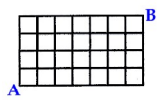
\includegraphics[scale=1.2]{kombin.PNG}
            Jika seseorang akan berjalan dari titik A ke titik B. Ada berapa banyak cara jalan terpendek 
        yang dapat dipilihnya ?
            
            \item (OSP 2003) Empat pasang suami istri menonton pagelaran orkestra. Tempat duduk mereka harus 
        dipisah antara kelompok suami dan kelompok istri. Untuk masing-masing kelompok disediakan 4
        buah tempat duduk bersebelahan dalam satu barisan. Ada berapa banyak cara memberikan 
        tempat duduk kepada mereka ?
        
            \item (OSK 2010) Banyaknya himpunan $X$ yang memenuhi 
        $$\{1,2,\dots,1000\} \subseteq X \subseteq \{1,2,\dots,2010\}.$$
        
            \item (OSP 2010) Bilangan enam digit $abcdef$ dengan $a > b > c \ge d > e > f$ ada sebanyak \dots
            
            \item (OSK 2017)
        	Sebuah hotel mempunyai kamar bernomor 000 sampai dengan 999. Hotel tersebut menerapkan
        aturan aneh sebagai berikut: jika suatu kamar berisi tamu, dan sembarang dua digit nomor kamar
        tersebut dipertukarkan tempatnya, maka diperoleh nomor kamar yang sama atau nomor kamar
        yang tidak berisi tamu. Maksimal banyaknya kamar yang berisi tamu adalah \dots
        
            \item (OSK 2012) Suatu set soal terdiri dari 10 soal pilihan B atau S dan 15 soal pilihan ganda dengan 4 pilihan. Seorang siswa menjawab semua soal dengan menebak jawaban secara acak. Tentukan probabilitas ia menjawab dengan benar hanya 2 soal.
            
            \item (OSK 2012) Misalkan terdapat 5 kartu dimana setiap kartu diberi nomor yang berbeda yaitu 2, 3, 4, 5, 6. Kartu-kartu tersebut kemudian dijajarkan dari kiri ke kanan secara acak sehingga berbentuk barisan. Berapa probabilitas bahwa banyaknya kartu yang dijajarkan dari kiri ke kanan dan ditempatkan pada tempat ke- $i$ akan lebih besar atau sama dengan $i$ untuk setiap $i$ dengan $1 \le i \le 5$ ?
            
            \item (OSK 2013) Suatu dadu ditos enam kali. Banyak cara memperoleh jumlah mata yang muncul 28 dengan tepat satu dadu muncul angka 6 adalah \dots
            
            \item (OSK 2013) Sepuluh kartu ditulis dengan angka satu sampai sepuluh (setiap kartu hanya terdapat satu angka dan tidak ada dua kartu yang memiliki angka yang sama). Kartu - kartu tersebut dimasukkan kedalam kotak dan diambil satu secara acak. Kemudian sebuah dadu dilempar. Probabilitas dari hasil kali angka pada kartu dan angka pada dadu menghasilkan bilangan kuadrat adalah \dots
            
            \item (OSK 2018) Diberikan satu koin yang tidak seimbang. Bila koin tersebut ditos satu kali, peluang muncul angka adalah $\frac{1}{4}$. Jika ditos $n$ kali, peluang muncul tepat dua angka sama dengan peluang muncul tepat tiga angka. Nilai $n$ adalah \dots
            
            \item (OSK 2017) Pada suatu kotak ada sekumpulan bola berwarna merah dan hitam yang secara keseluruhannya kurang dari 1000 bola. Misalkan diambil dua bola. Peluang terambilnya dua bola merah adalah $p$ dan peluang terambilnya dua bola hitam adalah $q$ dengan $p-q =\frac{23}{37}$. Selisih terbesar yang mungkin dari banyaknya bola merah dan hitam adalah \dots
            
            \item (OSK 2017) Terdapat enam anak, $A, B, C, D, E$ dan $F$, akan saling bertukar kado. Tidak ada yang menerima kadonya sendiri, dan kado dari $A$ diberikan kepada $B$. Banyaknya cara membagikan kado dengan cara demikian adalah \dots
            
             \item Carilah koefisien $x^4$ dari penjabaran $(x+1)^9$
                
                \item (OSK 2013) Koefisien $x^{2013}$ pada ekspansi
                $$(1+x)^{4026}+x(1+x)^{4025}+x^2(1+x)^{4024}+\dots x^{2013}(1+x)^{2013}$$
                adalah \dots
                
                \item Jika $S=(\sqrt{71}+1)^{71}-(\sqrt{71}-1)^{71}$ adalah bilangan bulat, carilah digit terakhir dari $S$
                \item Berapa banyak orang minimum yang harus hadir di suatu pesta sehingga dipastikan terdapat 3 orang yang lahir di bulan yang sama di pesta itu?
                
                \item Misalkan Naruko memilih $k$ buah bilangan dari himpunan $\{1,2,3,\dots,2016\}$ secara acak. Berapakah nilai $k$ terkecil sehingga Naruko pasti bisa mendapatkan setidaknya sepasang bilangan (dari $k$ bilangan itu) yang jika dijumlahkan hasilnya 2017?
                
                \item Suatu malam di rumah WonYoung terjadi pemadaman listrik. Karena WonYoung sangat malas, ia hanya ingin tidur dengan membawa banyak kaus kaki (hobi yang aneh :/). Ia mengambil kaus kaki dari lemari di ruangan yang sangat gelap. Lemari itu berisi 100 buah kaus kaki merah, 80 kaus kaki hijau, 60 kaus kaki biru, dan 40 kaus kaki hitam. WonYoung mengambil banyak kaus kaki tapi tidak bisa tahu warnanya. Berapa banyak kaus kaki paling sedikit yang perlu diambil sehingga dijamin terdapat setidaknya 10 pasang kaus kaki (dengan setiap pasang kaus kaki harus berwarna sama) ?
                
                \item (OSK 2011) Di lemari hanya ada 2 macam kaos kaki yaitu kaos kaki berwarna hitam dan putih. 
            Ali, Budi dan Candra berangkat di malam hari saat mati lampu dan mereka mengambil kaos kaki 
            secara acak di dalam lemari dalam kegelapan. Berapa kaos kaki minimal harus mereka ambil untuk 
            memastikan bahwa akan ada tiga pasang kaos kaki yang bisa mereka pakai ? (Sepasang kaos kaki harus 
            memiliki warna yang sama).
                
                \item Tandai satu buah kartu dengan angka 1, dua buah kartu dengan angka 2, tiga buah kartu dengan 
            angka satu hingga lima puluh buah kartu dengan angka 50. Semua kartu tersebut dimasukkan ke 
            dalam kotak. Berapa buah kartu minimal yang harus diambil agar dapat dipastikan terdapat sekurang-kurangnya 10 buah kartu dengan tanda angka yang sama 
            
                \item (OSK 2016)
            	Anak laki-laki dan anak perempuan yang berjumlah 48 orang duduk melingkar secara acak.
            Banyaknya minimum anak perempuan sehingga pasti ada enam anak perempuan yang duduk
            berdekatan tanpa diselingi anak laki-laki adalah \dots
        \end{enumerate}
    
    \section{Referensi}
        \begin{enumerate}
            \item Hermanto, Eddy. 2011. Diktat Pembinaan Olimpiade Matematika Dasar.
        \end{enumerate}
\end{document}


